\chapter{PX evaluation web application}
\label{ch:web_app}

A web application to manage \ac{PX} evaluations was developed using the Django framework \footnote{Django Project: \url{www.djangoproject.com}} (See \autoref{fig:dashboardApp}). The application contains ten modules that allow registering, updating and listing \ac{PX} evaluations for \acp{PREG} following the methodology presented in this chapter. The \autoref{fig:evaluationApp1} present the view of an evaluation being registered at the application and \autoref{fig:evaluationApp2} presents its detail view. To aim that, the following features are available:

\begin{enumerate}
    \item Registering, updating and listing evaluation aspects.
    \item Registering, updating and listing evaluation methods.
    \item Registering, updating and listing evaluation instruments.
    \item Registering, updating and listing evaluation questionnaires, following the standard presented in \autoref{ch:questionnaire} (See \autoref{fig:standardApp}).
    \item Registering, updating and listing \acp{PREG} following the characterising approach presented in \autoref{sec:characterising} (See \autoref{fig:characterisingApp}).
    \item Registering, updating and listing rehabilitation constraints.
    \item Registering, updating and listing rehabilitation associated tasks (e.g, supervising and motivating).
    \item Registering, updating and listing interaction devices and technologies.
    \item Registering, updating and listing rehabilitation movements and configuration parameters.
    \item Registering, updating and listing impairments.
    \item Registering, updating and listing resources (e.g. evaluation reports or protocols).
    \item A wiki to access to articles explaining the \ac{PX} evaluation methodology and the questionnaire standard.
\end{enumerate}

The application was developed using agile practices such as the use of a task-board, user stories and issues. The development process was managed using the ZenHub \footnote{ZenHub: \url{https://www.zenhub.com/}} application and the code versioning was managed using git \footnote{Git: \url{https://git-scm.com/}} and GitHub \footnote{GitHub: \url{https://github.com/}}. The source code of the application is available online \footnote{Source code repository: \url{https://github.com/edwingamboa/rehab-exergames-px-app}}.

\begin{figure}[bth]
\myfloatalign
{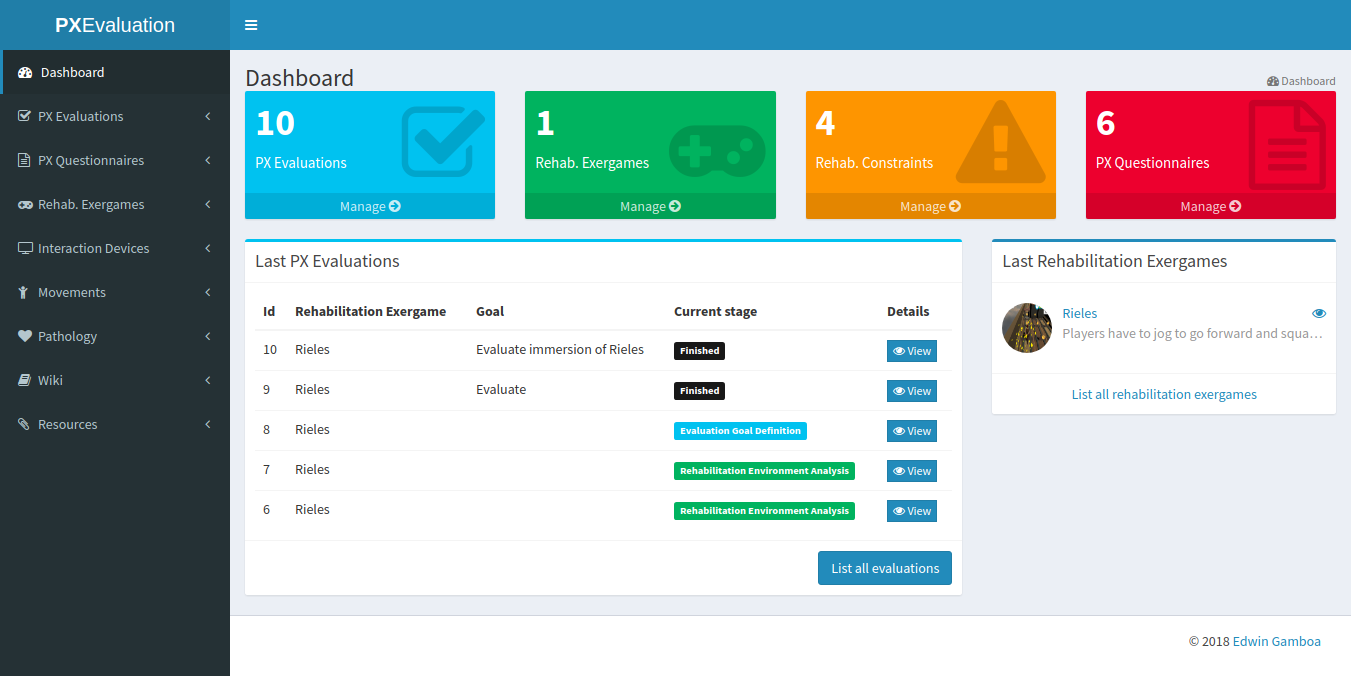
\includegraphics[width=\linewidth]{gfx/app/dashboardApp}} \quad
\caption{Dashboard of the \ac{PX} evaluation application}\label{fig:dashboardApp}
\end{figure}

\begin{figure}[bth]
\myfloatalign
{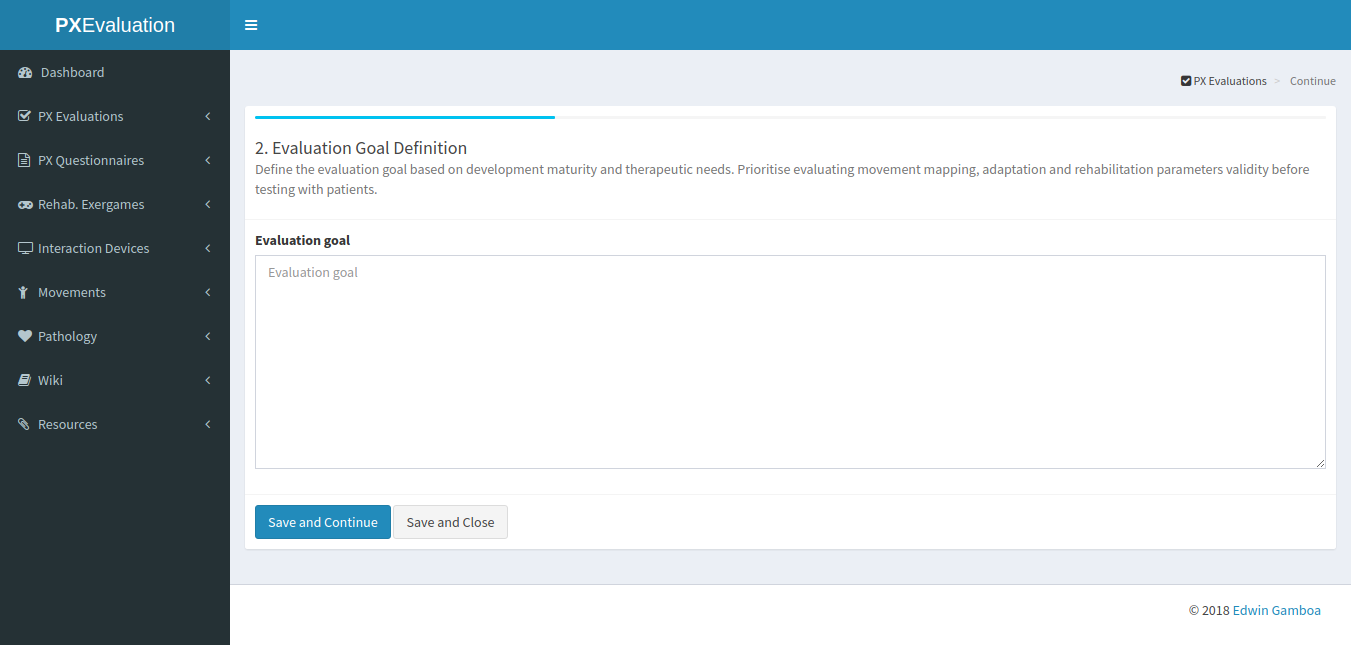
\includegraphics[width=\linewidth]{gfx/app/evaluationApp1}} \quad
\caption{Register view of an evaluation at the \ac{PX} evaluation application}\label{fig:evaluationApp1}
\end{figure}

\begin{figure}[bth]
\myfloatalign
{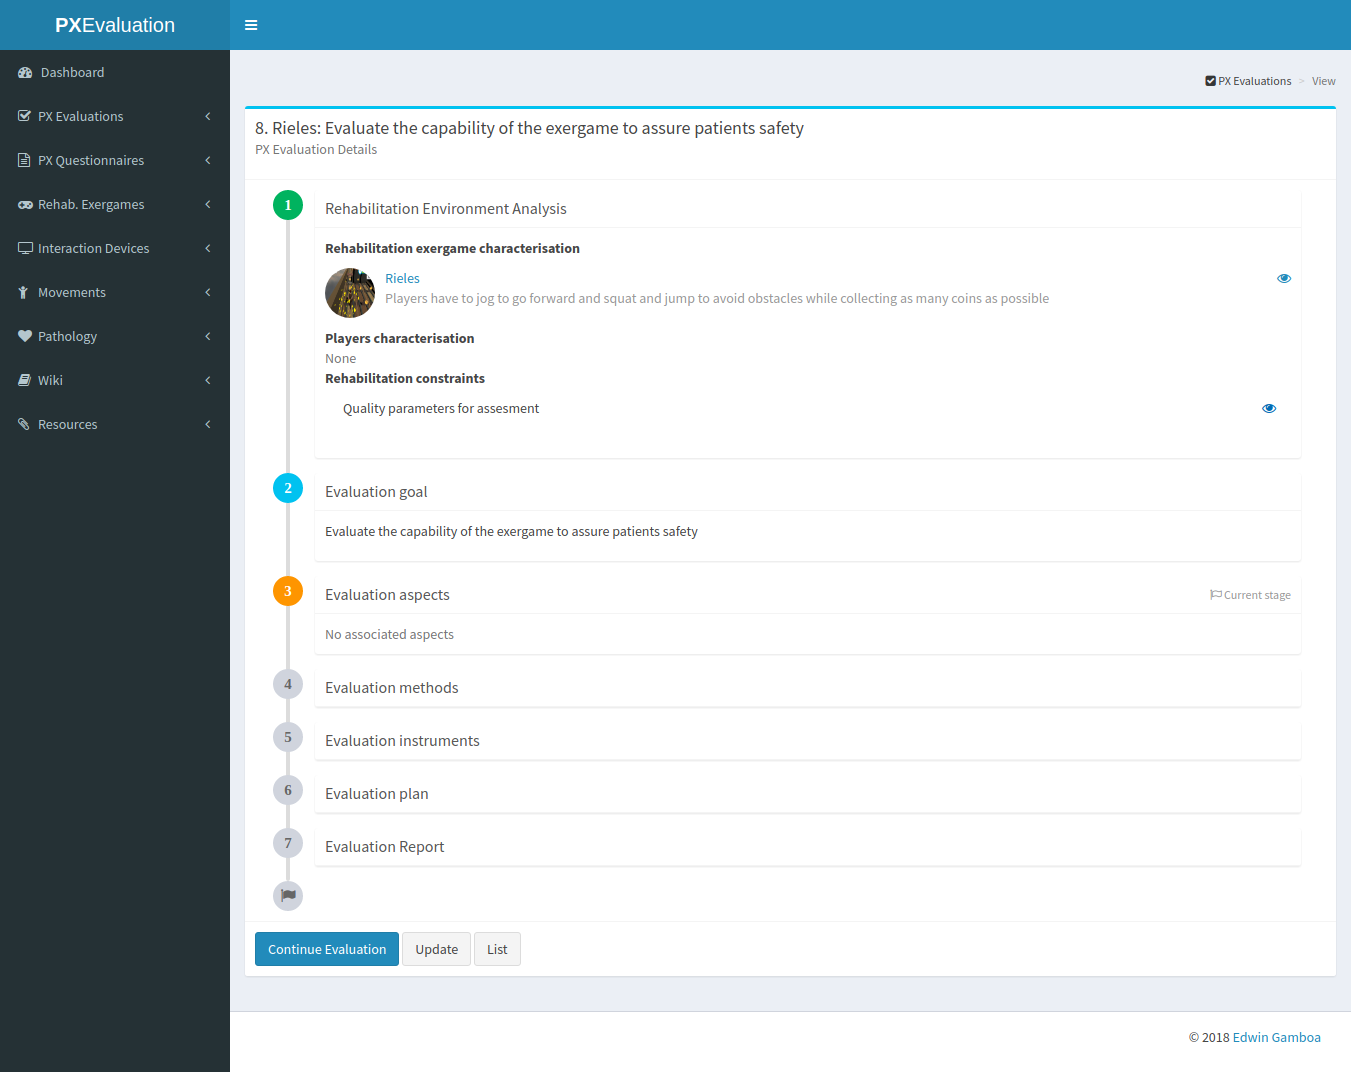
\includegraphics[width=\linewidth]{gfx/app/evaluationApp2}} \quad
\caption{Detail view of an evaluation at the \ac{PX} evaluation application}\label{fig:evaluationApp2}
\end{figure}


\begin{figure}[bth]
\myfloatalign
{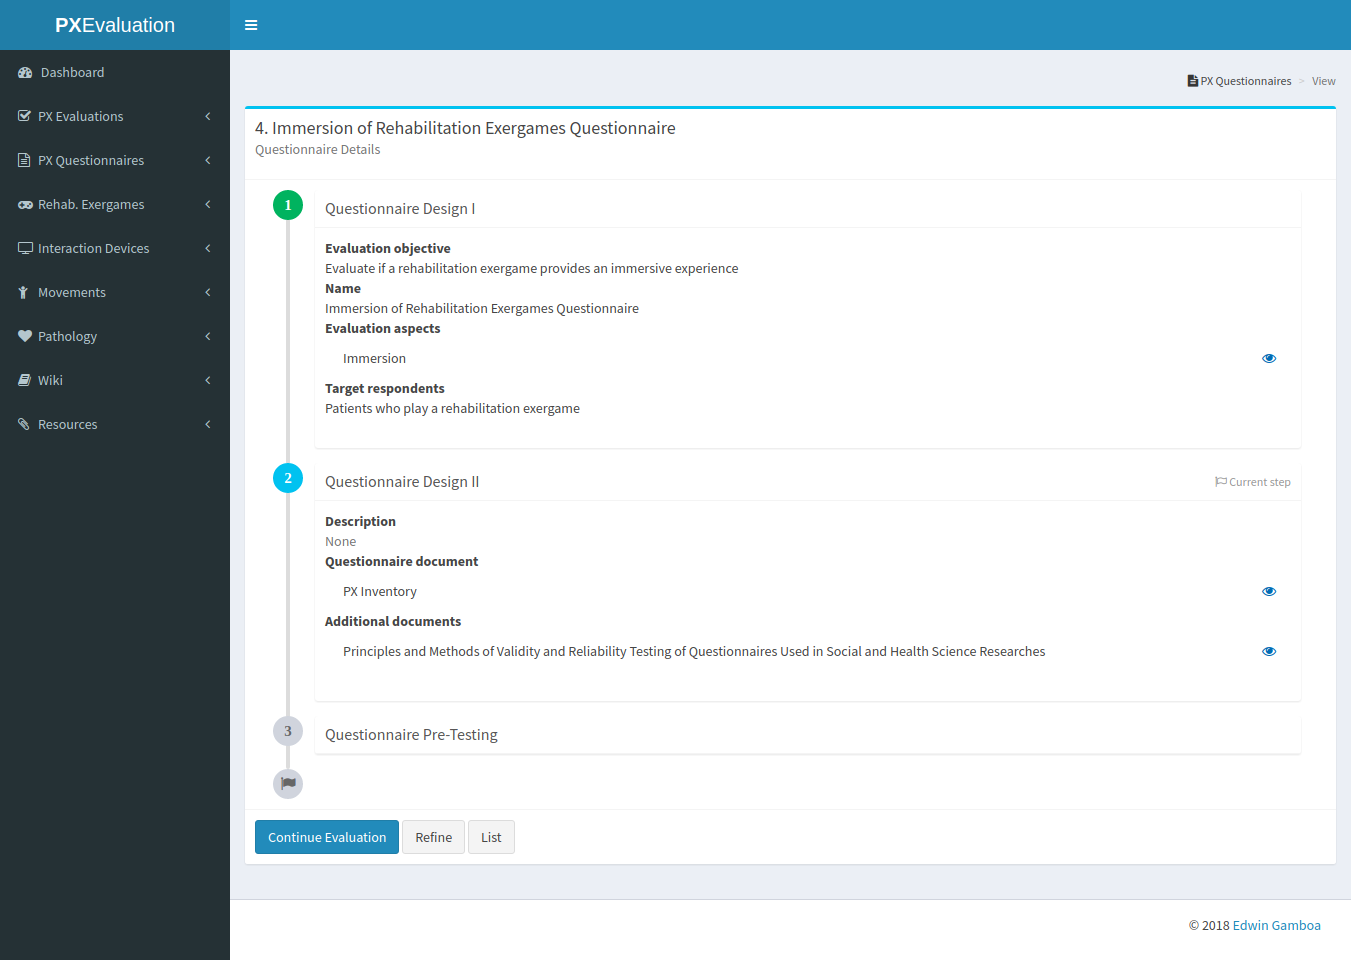
\includegraphics[width=\linewidth]{gfx/app/standardApp}} \quad
\caption{Detail view of a standard being developed at the \ac{PX} evaluation application}\label{fig:standardApp}
\end{figure}

\begin{figure}[bth]
\myfloatalign
{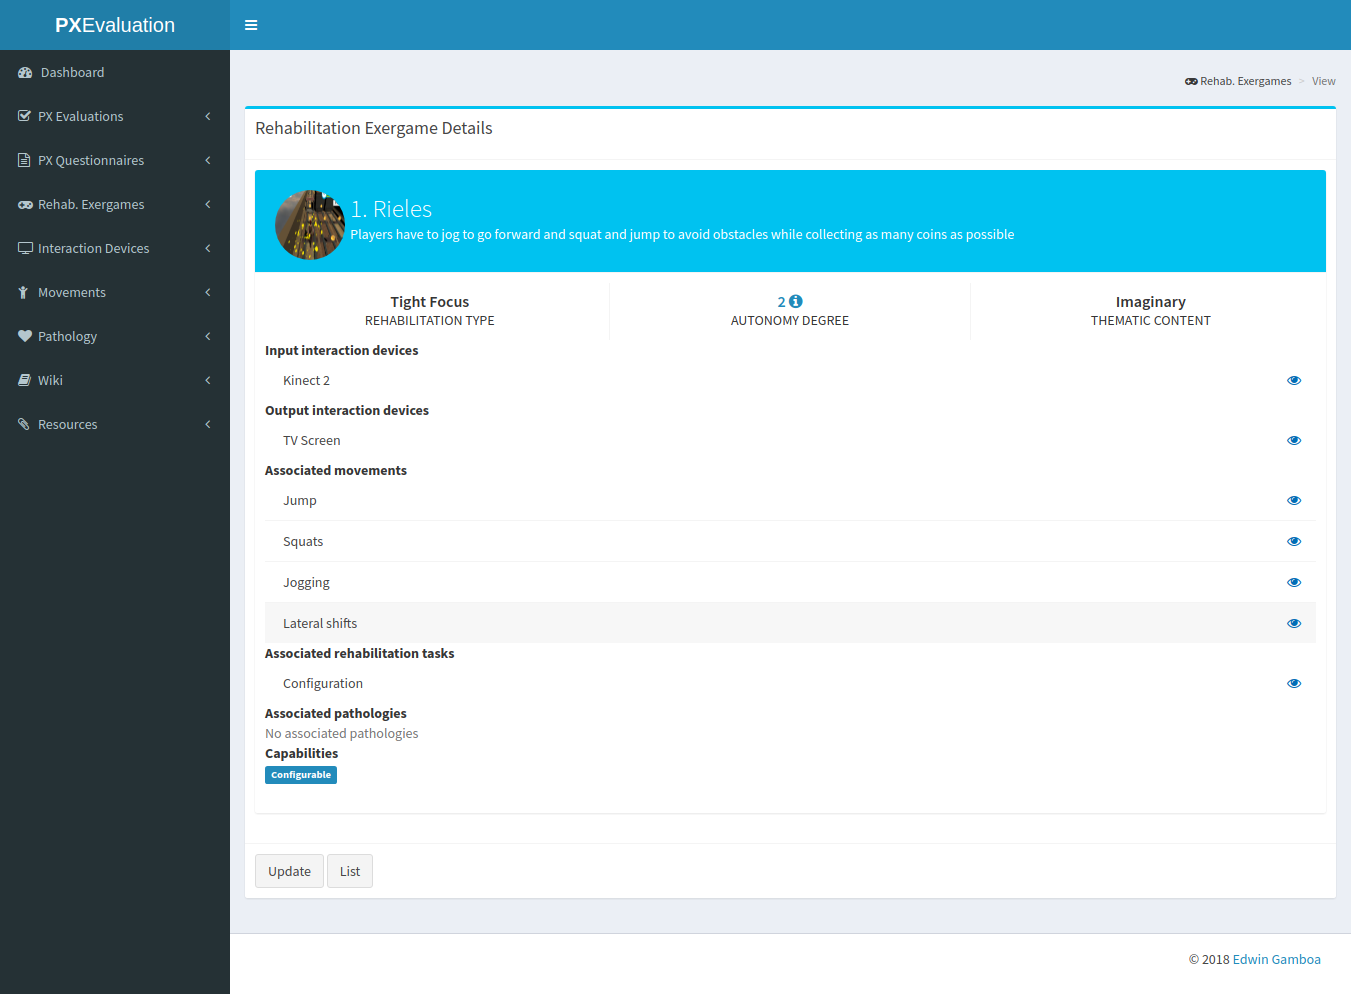
\includegraphics[width=\linewidth]{gfx/app/characterisingApp}} \quad
\caption{Detail view of a \ac{PREG} characterisation at the \ac{PX} evaluation application}\label{fig:characterisingApp}
\end{figure}

\section{Conclusion}
In this chapter, we presented a methodology for evaluating PX in \acp{PREG}. Our proposal is based on the model presented on \autoref{ch:model}; highlighting crucial aspects to be evaluated before, during and after interaction between a patient, a context and a \ac{PREG} occurs. Since the methodology is based on a \ac{PX} model for \acp{PREG}, it allows performing evaluations that meet the constraints that the rehabilitation environment may impose. It requires evaluators to characterise \acp{PREG} considering its therapeutic goal, to define users profile considering its characteristics as patients and analysing the involved rehabilitation environment. Thus, our approach differs from other evaluations in which \acp{PREG}s are evaluated considering only motivation, enjoyment or usability \autocite{Brokaw2015,Burke2009,Cameirao2010,jansen2013serious,Ni2014}.

The proposed methodology is intended to be used iteratively to perform a comprehensive evaluation. However, it was built based on a model designed using a qualitative approach, thereby limiting its generalisation. Thus, we still need to use the methodology extensively to identify gaps and additional constraints that should be considered. This process would allow us to validate the relevance of the highlighted stages in real use cases.

Finally, the proposed methodology may be extended or adapted to other domains in which entertainment is not the main goal. In that case, the domain constraints should be identified to define a set of relevant aspects, methods and instruments to be employed during \ac{PX} evaluation.
